% Auto-generated by analysis/semantic/oncoco/make_hmm_phase_tikz.py -- do not edit by hand.
\documentclass[border=1pt,10pt]{standalone}
\usepackage[T1]{fontenc}
\usepackage[scaled=0.92]{helvet}
\renewcommand{\familydefault}{\sfdefault}
\usepackage{sansmath}
\sansmath
\usepackage{tikz}
\usetikzlibrary{arrows.meta,positioning,calc}

\definecolor{cReal}{HTML}{2C6E63}
\definecolor{cRP}{HTML}{4A6E9B}
\definecolor{cLLM}{HTML}{C0503C}
\definecolor{cInk}{HTML}{1F2328}
\definecolor{cMute}{HTML}{70757D}
\definecolor{cRule}{HTML}{CFD4DA}
\definecolor{cPanel}{HTML}{FBFBFC}
\definecolor{cBand}{HTML}{E5E9EE}

\begin{document}
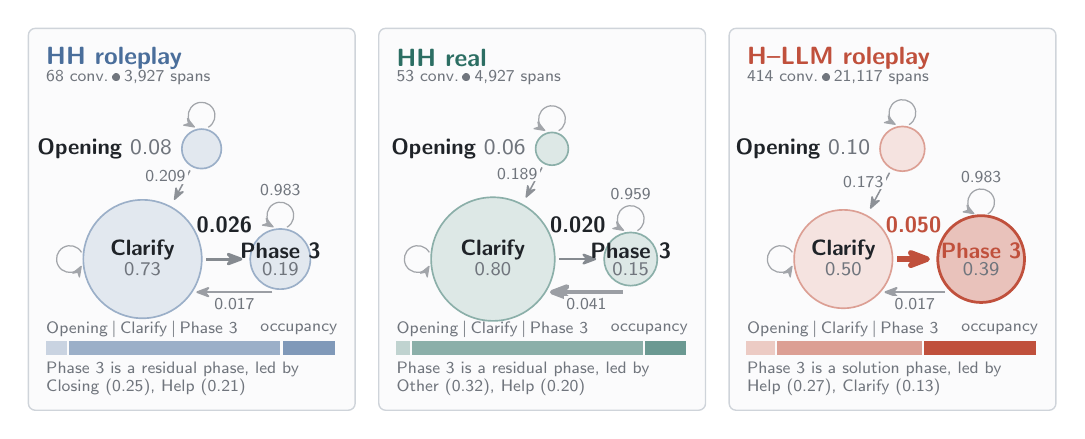
\begin{tikzpicture}[x=1cm,y=1cm,>={Stealth[round]}]
\path (0,0) rectangle (13.05,4.85);

  % ---------------- HH roleplay
  \begin{scope}[shift={(0.00,0)}]
  \draw[rounded corners=2.5pt, draw=cRule, fill=cPanel, line width=0.5pt] (0,0) rectangle (4.15,4.85);
  \node[anchor=west, font=\fontsize{9.5}{11}\selectfont\bfseries, text=cRP, inner sep=0pt] at (0.22,4.47) {HH roleplay};
  \node[anchor=west, font=\fontsize{6.0}{7.0}\selectfont, text=cMute, inner sep=0pt] at (0.22,4.23) {68 conv.\,\textbullet\,3{,}927 spans};
  \draw[->, cMute!80, line width=0.55pt] (2.053,3.046) -- (1.852,2.671);
  \node[font=\fontsize{6.0}{7.0}\selectfont, text=cMute, fill=cPanel, inner sep=0.8pt] at (1.741,2.972) {0.209};
  \draw[->, cMute!85, line width=1.06pt] (2.262,1.920) -- (2.718,1.920);
  \node[font=\fontsize{7.9}{9.1}\selectfont\bfseries, text=cInk, fill=cPanel, inner sep=1.0pt] at (2.490,2.360) {0.026};
  \draw[->, cMute!70, line width=0.67pt] (3.100,1.500) -- (2.134,1.500);
  \node[font=\fontsize{6.0}{7.0}\selectfont, text=cMute, fill=cPanel, inner sep=0.8pt] at (2.617,1.350) {0.017};
  \fill[cRP!16] (2.20,3.32) circle (0.251);
  \draw[cRP!55, line width=0.6pt] (2.20,3.32) circle (0.251);
  \node[anchor=east, font=\fontsize{7.7}{8.9}\selectfont, inner sep=0pt] at (1.829,3.32) {\textcolor{cInk}{\bfseries Opening}~\textcolor{cMute}{0.08}};
  \fill[cRP!16] (1.45,1.92) circle (0.752);
  \draw[cRP!55, line width=0.6pt] (1.45,1.92) circle (0.752);
  \node[font=\fontsize{7.7}{8.9}\selectfont\bfseries, text=cInk, inner sep=0pt] at (1.45,2.03) {Clarify};
  \node[font=\fontsize{6.7}{7.9}\selectfont, text=cMute, inner sep=0pt] at (1.45,1.79) {0.73};
  \fill[cRP!16] (3.20,1.92) circle (0.382);
  \draw[cRP!55, line width=0.6pt] (3.20,1.92) circle (0.382);
  \node[font=\fontsize{7.7}{8.9}\selectfont\bfseries, text=cInk, inner sep=0pt] at (3.20,2.03) {Phase 3};
  \node[font=\fontsize{6.7}{7.9}\selectfont, text=cMute, inner sep=0pt] at (3.20,1.79) {0.19};
  \draw[->, cMute!65, line width=0.45pt] (2.285,3.594) arc[start angle=-60, delta angle=300, radius=0.17];
  \draw[->, cMute!65, line width=0.45pt] (0.675,2.005) arc[start angle=30, delta angle=300, radius=0.17];
  \draw[->, cMute!65, line width=0.45pt] (3.285,2.325) arc[start angle=-60, delta angle=300, radius=0.17];
  \node[font=\fontsize{5.8}{6.7}\selectfont, text=cMute, inner sep=1.0pt, anchor=south] at (3.200,2.682) {0.983};
  \fill[cRP!30] (0.220,0.70) rectangle (0.492,0.88);
  \fill[cRP!55] (0.522,0.70) rectangle (3.202,0.88);
  \fill[cRP!70] (3.232,0.70) rectangle (3.900,0.88);
  \node[anchor=east, font=\fontsize{5.8}{6.7}\selectfont, text=cMute, inner sep=0pt] at (3.93,1.03) {occupancy};
  \node[anchor=west, font=\fontsize{5.8}{6.7}\selectfont, text=cMute, inner sep=0pt] at (0.22,1.03) {Opening\,\textbar\,Clarify\,\textbar\,Phase 3};
  \node[anchor=west, font=\fontsize{5.8}{6.7}\selectfont, text=cMute, inner sep=0pt, align=left, text width=3.71cm] at (0.22,0.40) {Phase 3 is a residual phase, led by Closing (0.25), Help (0.21)};
  \end{scope}

  % ---------------- HH real
  \begin{scope}[shift={(4.45,0)}]
  \draw[rounded corners=2.5pt, draw=cRule, fill=cPanel, line width=0.5pt] (0,0) rectangle (4.15,4.85);
  \node[anchor=west, font=\fontsize{9.5}{11}\selectfont\bfseries, text=cReal, inner sep=0pt] at (0.22,4.47) {HH real};
  \node[anchor=west, font=\fontsize{6.0}{7.0}\selectfont, text=cMute, inner sep=0pt] at (0.22,4.23) {53 conv.\,\textbullet\,4{,}927 spans};
  \draw[->, cMute!80, line width=0.55pt] (2.074,3.084) -- (1.868,2.700);
  \node[font=\fontsize{6.0}{7.0}\selectfont, text=cMute, fill=cPanel, inner sep=0.8pt] at (1.759,3.006) {0.189};
  \draw[->, cMute!85, line width=0.80pt] (2.295,1.920) -- (2.762,1.920);
  \node[font=\fontsize{7.9}{9.1}\selectfont\bfseries, text=cInk, fill=cPanel, inner sep=1.0pt] at (2.529,2.360) {0.020};
  \draw[->, cMute!70, line width=1.63pt] (3.100,1.500) -- (2.174,1.500);
  \node[font=\fontsize{6.0}{7.0}\selectfont, text=cMute, fill=cPanel, inner sep=0.8pt] at (2.637,1.350) {0.041};
  \fill[cReal!16] (2.20,3.32) circle (0.208);
  \draw[cReal!55, line width=0.6pt] (2.20,3.32) circle (0.208);
  \node[anchor=east, font=\fontsize{7.7}{8.9}\selectfont, inner sep=0pt] at (1.872,3.32) {\textcolor{cInk}{\bfseries Opening}~\textcolor{cMute}{0.06}};
  \fill[cReal!16] (1.45,1.92) circle (0.785);
  \draw[cReal!55, line width=0.6pt] (1.45,1.92) circle (0.785);
  \node[font=\fontsize{7.7}{8.9}\selectfont\bfseries, text=cInk, inner sep=0pt] at (1.45,2.03) {Clarify};
  \node[font=\fontsize{6.7}{7.9}\selectfont, text=cMute, inner sep=0pt] at (1.45,1.79) {0.80};
  \fill[cReal!16] (3.20,1.92) circle (0.338);
  \draw[cReal!55, line width=0.6pt] (3.20,1.92) circle (0.338);
  \node[font=\fontsize{7.7}{8.9}\selectfont\bfseries, text=cInk, inner sep=0pt] at (3.20,2.03) {Phase 3};
  \node[font=\fontsize{6.7}{7.9}\selectfont, text=cMute, inner sep=0pt] at (3.20,1.79) {0.15};
  \draw[->, cMute!65, line width=0.45pt] (2.285,3.550) arc[start angle=-60, delta angle=300, radius=0.17];
  \draw[->, cMute!65, line width=0.45pt] (0.642,2.005) arc[start angle=30, delta angle=300, radius=0.17];
  \draw[->, cMute!65, line width=0.45pt] (3.285,2.281) arc[start angle=-60, delta angle=300, radius=0.17];
  \node[font=\fontsize{5.8}{6.7}\selectfont, text=cMute, inner sep=1.0pt, anchor=south] at (3.200,2.638) {0.959};
  \fill[cReal!30] (0.220,0.70) rectangle (0.396,0.88);
  \fill[cReal!55] (0.426,0.70) rectangle (3.352,0.88);
  \fill[cReal!70] (3.382,0.70) rectangle (3.900,0.88);
  \node[anchor=east, font=\fontsize{5.8}{6.7}\selectfont, text=cMute, inner sep=0pt] at (3.93,1.03) {occupancy};
  \node[anchor=west, font=\fontsize{5.8}{6.7}\selectfont, text=cMute, inner sep=0pt] at (0.22,1.03) {Opening\,\textbar\,Clarify\,\textbar\,Phase 3};
  \node[anchor=west, font=\fontsize{5.8}{6.7}\selectfont, text=cMute, inner sep=0pt, align=left, text width=3.71cm] at (0.22,0.40) {Phase 3 is a residual phase, led by Other (0.32), Help (0.20)};
  \end{scope}

  % ---------------- H--LLM roleplay
  \begin{scope}[shift={(8.90,0)}]
  \draw[rounded corners=2.5pt, draw=cRule, fill=cPanel, line width=0.5pt] (0,0) rectangle (4.15,4.85);
  \node[anchor=west, font=\fontsize{9.5}{11}\selectfont\bfseries, text=cLLM, inner sep=0pt] at (0.22,4.47) {H--LLM roleplay};
  \node[anchor=west, font=\fontsize{6.0}{7.0}\selectfont, text=cMute, inner sep=0pt] at (0.22,4.23) {414 conv.\,\textbullet\,21{,}117 spans};
  \draw[->, cMute!80, line width=0.55pt] (2.037,3.017) -- (1.792,2.559);
  \node[font=\fontsize{6.0}{7.0}\selectfont, text=cMute, fill=cPanel, inner sep=0.8pt] at (1.703,2.901) {0.173};
  \draw[->, cLLM, line width=1.98pt] (2.135,1.920) -- (2.549,1.920);
  \node[font=\fontsize{7.9}{9.1}\selectfont\bfseries, text=cLLM, fill=cPanel, inner sep=1.0pt] at (2.342,2.360) {0.050};
  \draw[->, cMute!70, line width=0.69pt] (2.744,1.500) -- (1.973,1.500);
  \node[font=\fontsize{6.0}{7.0}\selectfont, text=cMute, fill=cPanel, inner sep=0.8pt] at (2.358,1.350) {0.017};
  \fill[cLLM!16] (2.20,3.32) circle (0.284);
  \draw[cLLM!55, line width=0.6pt] (2.20,3.32) circle (0.284);
  \node[anchor=east, font=\fontsize{7.7}{8.9}\selectfont, inner sep=0pt] at (1.796,3.32) {\textcolor{cInk}{\bfseries Opening}~\textcolor{cMute}{0.10}};
  \fill[cLLM!16] (1.45,1.92) circle (0.625);
  \draw[cLLM!55, line width=0.6pt] (1.45,1.92) circle (0.625);
  \node[font=\fontsize{7.7}{8.9}\selectfont\bfseries, text=cInk, inner sep=0pt] at (1.45,2.03) {Clarify};
  \node[font=\fontsize{6.7}{7.9}\selectfont, text=cMute, inner sep=0pt] at (1.45,1.79) {0.50};
  \fill[cLLM!35] (3.20,1.92) circle (0.551);
  \draw[cLLM!100, line width=1.0pt] (3.20,1.92) circle (0.551);
  \node[font=\fontsize{7.7}{8.9}\selectfont\bfseries, text=cLLM, inner sep=0pt] at (3.20,2.03) {Phase 3};
  \node[font=\fontsize{6.7}{7.9}\selectfont, text=cMute, inner sep=0pt] at (3.20,1.79) {0.39};
  \draw[->, cMute!65, line width=0.45pt] (2.285,3.627) arc[start angle=-60, delta angle=300, radius=0.17];
  \draw[->, cMute!65, line width=0.45pt] (0.802,2.005) arc[start angle=30, delta angle=300, radius=0.17];
  \draw[->, cMute!65, line width=0.45pt] (3.285,2.493) arc[start angle=-60, delta angle=300, radius=0.17];
  \node[font=\fontsize{5.8}{6.7}\selectfont, text=cMute, inner sep=1.0pt, anchor=south] at (3.200,2.851) {0.983};
  \fill[cLLM!30] (0.220,0.70) rectangle (0.577,0.88);
  \fill[cLLM!55] (0.607,0.70) rectangle (2.447,0.88);
  \fill[cLLM!100] (2.477,0.70) rectangle (3.900,0.88);
  \node[anchor=east, font=\fontsize{5.8}{6.7}\selectfont, text=cMute, inner sep=0pt] at (3.93,1.03) {occupancy};
  \node[anchor=west, font=\fontsize{5.8}{6.7}\selectfont, text=cMute, inner sep=0pt] at (0.22,1.03) {Opening\,\textbar\,Clarify\,\textbar\,Phase 3};
  \node[anchor=west, font=\fontsize{5.8}{6.7}\selectfont, text=cMute, inner sep=0pt, align=left, text width=3.71cm] at (0.22,0.40) {Phase 3 is a solution phase, led by Help (0.27), Clarify (0.13)};
  \end{scope}
\end{tikzpicture}
\end{document}
